\documentclass[tikz,border=6pt]{standalone}
\usepackage{amsmath}
\usetikzlibrary{arrows.meta,positioning,calc,fit}

\begin{document}
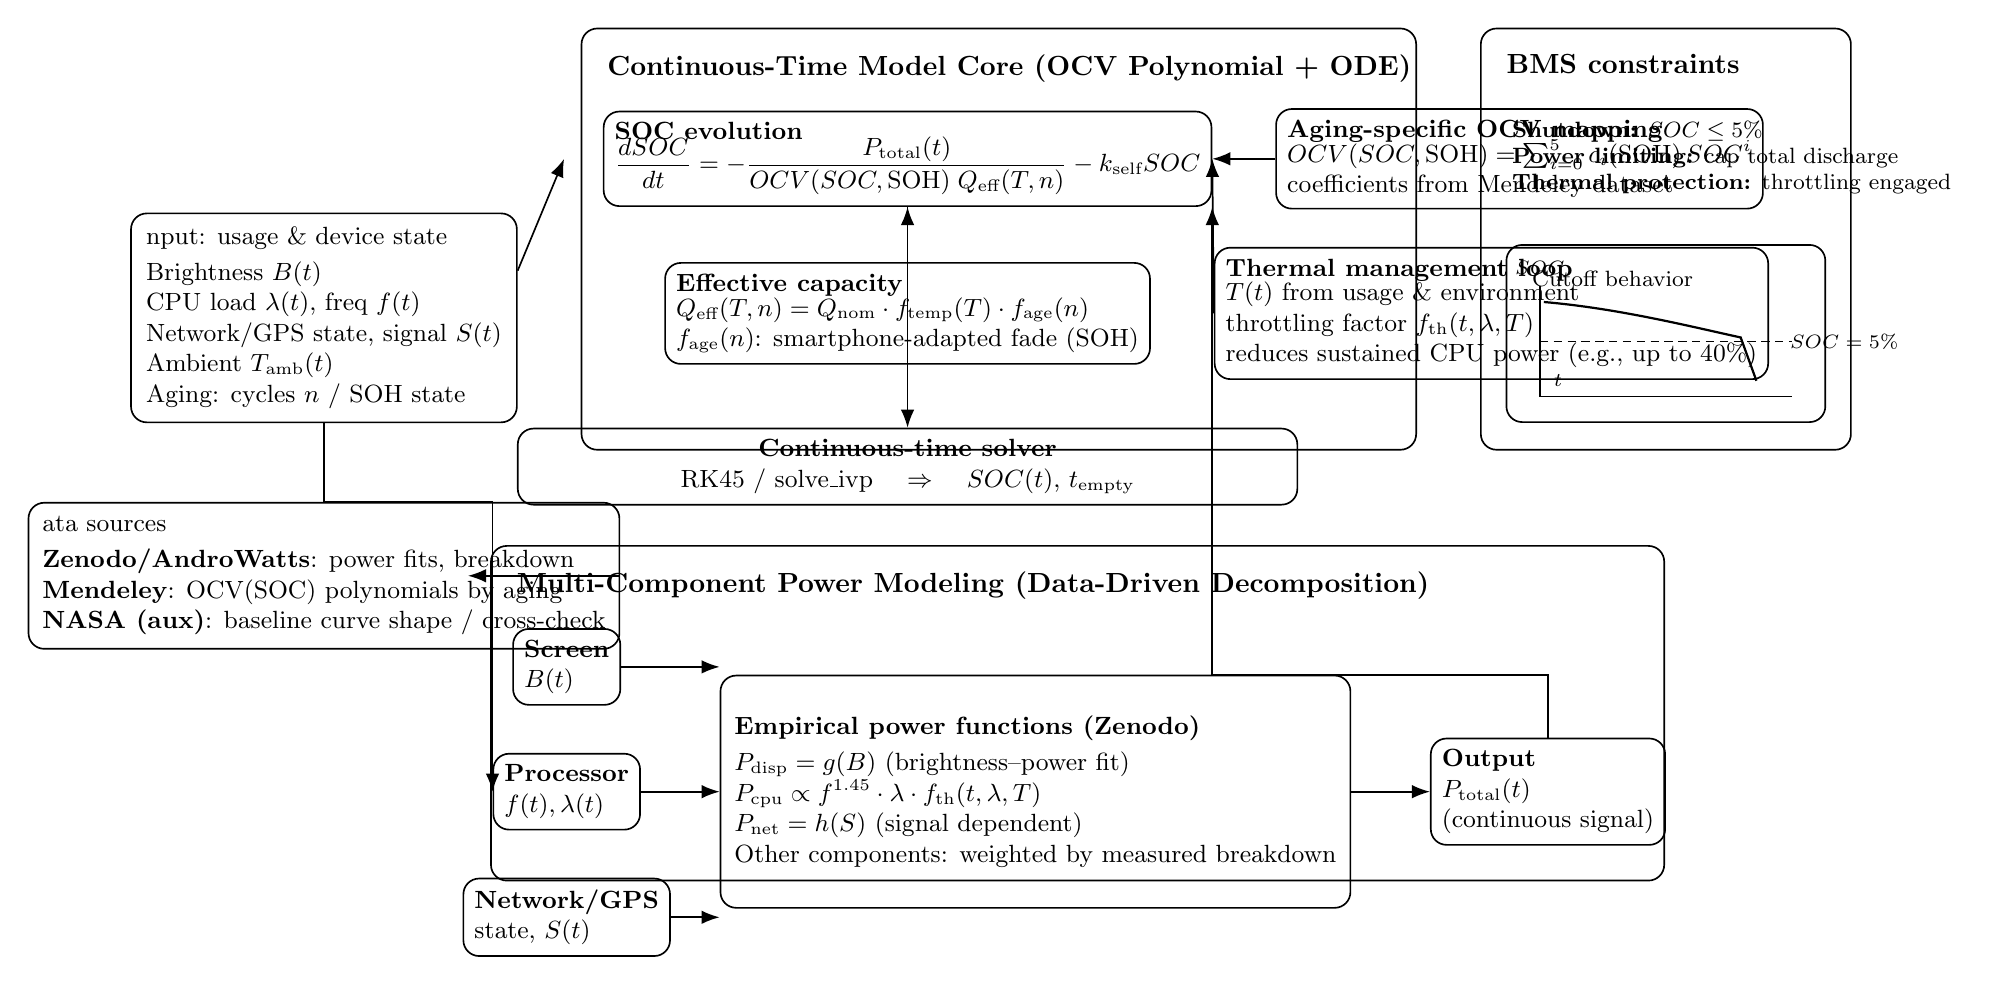
\begin{tikzpicture}[
  font=\small,
  line width=0.6pt,
  >={Latex[length=2.3mm]},
  box/.style={draw, rounded corners=2mm, align=left, inner sep=5pt},
  smallbox/.style={draw, rounded corners=2mm, align=center, inner sep=4pt},
  title/.style={font=\bfseries},
  note/.style={font=\footnotesize, align=left},
  arrow/.style={->},
  dashed line/.style={densely dashed},
]

% =========================
% Left: inputs
% =========================
\node[box, minimum width=4.9cm] (input) {
  {\title Input: usage \& device state}\\[2pt]
  Brightness $B(t)$\\
  CPU load $\lambda(t)$, freq $f(t)$\\
  Network/GPS state, signal $S(t)$\\
  Ambient $T_{\text{amb}}(t)$\\
  Aging: cycles $n$ / SOH state
};

% =========================
% Data sources box
% =========================
\node[box, minimum width=4.9cm, below=10mm of input] (data) {
  {\title Data sources}\\[2pt]
  \textbf{Zenodo/AndroWatts}: power fits, breakdown\\
  \textbf{Mendeley}: OCV(SOC) polynomials by aging\\
  \textbf{NASA (aux)}: baseline curve shape / cross-check
};

% =========================
% Top center: core container
% =========================
\node[box, minimum width=10.6cm, minimum height=5.35cm, right=8mm of input, yshift=10mm] (core) {};
\node[title, anchor=north west] at ([xshift=6pt,yshift=-6pt]core.north west)
{Continuous-Time Model Core (OCV Polynomial + ODE)};

% ODE box
\node[smallbox, anchor=north west, align=left] (ode) at ([xshift=8pt,yshift=-30pt]core.north west) {
  \textbf{SOC evolution}\\[-2pt]
  $\displaystyle \frac{dSOC}{dt}
  =-\frac{P_{\text{total}}(t)}{OCV(SOC,\text{SOH})\;Q_{\text{eff}}(T,n)}
  -k_{\text{self}}SOC$
};

% OCV mapping
\node[smallbox, right=8mm of ode, align=left] (ocv) {
  \textbf{Aging-specific OCV mapping}\\[-2pt]
  $OCV(SOC,\text{SOH})=\sum_{i=0}^{5} c_i(\text{SOH})\,SOC^i$\\
  coefficients from Mendeley dataset
};

% Qeff
\node[smallbox, below=7mm of ode, align=left] (qeff) {
  \textbf{Effective capacity}\\[-2pt]
  $Q_{\text{eff}}(T,n)=Q_{\text{nom}}\cdot f_{\text{temp}}(T)\cdot f_{\text{age}}(n)$\\
  $f_{\text{age}}(n)$: smartphone-adapted fade (SOH)
};

% Thermal feedback
\node[smallbox, right=8mm of qeff, align=left] (thermal) {
  \textbf{Thermal management loop}\\[-2pt]
  $T(t)$ from usage \& environment\\
  throttling factor $f_{\text{th}}(t,\lambda,T)$\\
  reduces sustained CPU power (e.g., up to 40\%)
};

% solver
\node[smallbox, minimum width=9.9cm, below=8mm of qeff] (solver) {
  \textbf{Continuous-time solver}\\
  RK45 / solve\_ivp \quad $\Rightarrow$ \quad $SOC(t)$, $t_{\text{empty}}$
};

% arrows inside core
\draw[arrow] (input.east) ++(0,6mm) -- ([xshift=-6pt]core.west |- ode.west);
\draw[arrow] (ocv.west) -- (ode.east |- ocv.west);
\draw[arrow] (qeff.north) -- (ode.south);
\draw[arrow] (thermal.west) -- (ode.east);
\draw[arrow] (ode.south) -- (solver.north);

% =========================
% Right: BMS constraints panel + cutoff plot
% =========================
\node[box, minimum width=4.7cm, minimum height=5.35cm, right=8mm of core] (bms) {};
\node[title, anchor=north west] at ([xshift=6pt,yshift=-6pt]bms.north west)
{BMS constraints};

\node[note, anchor=north west] at ([xshift=8pt,yshift=-30pt]bms.north west) (bmslist) {
  \textbf{Shutdown:} $SOC \le 5\%$\\
  \textbf{Power limiting:} cap total discharge\\
  \textbf{Thermal protection:} throttling engaged
};

\node[smallbox, minimum width=4.05cm, minimum height=2.25cm, anchor=south] (plot) at ([yshift=10pt]bms.south) {};
\node[note, anchor=north west] at ([xshift=6pt,yshift=-6pt]plot.north west) {Cutoff behavior};

% axes
\draw[line width=0.5pt] ([xshift=-1.6cm,yshift=-0.8cm]plot.center) -- ++(0,1.4cm);
\draw[line width=0.5pt] ([xshift=-1.6cm,yshift=-0.8cm]plot.center) -- ++(3.2cm,0);

% threshold line
\draw[dashed line] ([xshift=-1.6cm,yshift=-0.1cm]plot.center) -- ++(3.2cm,0);
\node[font=\scriptsize, anchor=west] at ([xshift=1.45cm,yshift=-0.1cm]plot.center) {$SOC=5\%$};

% curve
\draw[line width=0.8pt]
  ([xshift=-1.55cm,yshift=0.40cm]plot.center)
  .. controls ([xshift=-0.6cm,yshift=0.32cm]plot.center)
  and ([xshift=0.35cm,yshift=0.08cm]plot.center)
  .. ([xshift=0.95cm,yshift=-0.05cm]plot.center)
  -- ([xshift=1.15cm,yshift=-0.60cm]plot.center);

\node[font=\scriptsize, anchor=south west] at ([xshift=-1.55cm,yshift=-0.8cm]plot.center) {$t$};
\node[font=\scriptsize, anchor=south] at ([xshift=-1.6cm,yshift=0.62cm]plot.center) {$SOC$};

% =========================
% Bottom: multi-component power decomposition
% =========================
\node[box, minimum width=14.9cm, minimum height=4.25cm, below=12mm of core, xshift=1.0cm] (load) {};
\node[title, anchor=north west] at ([xshift=6pt,yshift=-6pt]load.north west)
{Multi-Component Power Modeling (Data-Driven Decomposition)};

\node[smallbox, align=left, anchor=north west] (u1) at ([xshift=8pt,yshift=-30pt]load.north west) {
  \textbf{Screen}\\
  $B(t)$
};
\node[smallbox, align=left, below=6mm of u1] (u2) {
  \textbf{Processor}\\
  $f(t),\lambda(t)$
};
\node[smallbox, align=left, below=6mm of u2] (u3) {
  \textbf{Network/GPS}\\
  state, $S(t)$
};

\node[smallbox, minimum width=8.0cm, minimum height=2.95cm, right=10mm of u2, align=left] (decomp) {
  \textbf{Empirical power functions (Zenodo)}\\[2pt]
  $P_{\text{disp}}=g(B)$ (brightness--power fit)\\
  $P_{\text{cpu}}\propto f^{1.45}\cdot \lambda \cdot f_{\text{th}}(t,\lambda,T)$\\
  $P_{\text{net}}=h(S)$ (signal dependent)\\
  Other components: weighted by measured breakdown
};

\node[smallbox, align=left, right=10mm of decomp] (ptotal) {
  \textbf{Output}\\
  $P_{\text{total}}(t)$\\
  (continuous signal)
};

\draw[arrow] (u1.east) -- (decomp.west |- u1.east);
\draw[arrow] (u2.east) -- (decomp.west);
\draw[arrow] (u3.east) -- (decomp.west |- u3.east);
\draw[arrow] (decomp.east) -- (ptotal.west);

% connect P_total up to ODE
\draw[arrow] (ptotal.north) -- ++(0,8mm) -| (ode.south east);

% connect data sources into load model
\draw[arrow] (data.east) -- ([xshift=-8pt]load.west |- data.east);

% connect input down to load inputs
\draw[arrow] (input.south) -- ++(0,-10mm) -| (u2.west);

\end{tikzpicture}
\end{document}
